\documentclass[10pt]{beamer}

\usetheme{metropolis}
\usepackage{appendixnumberbeamer}

\usepackage{booktabs}
\usepackage[scale=2]{ccicons}

\usepackage{pgfplots}
\usepgfplotslibrary{dateplot}

\usepackage{xspace}
\newcommand{\themename}{\textbf{\textsc{metropolis}}\xspace}

\title{Weekly Meeting}
\subtitle{What I did this week}
\date{\today}
\author{Yanchen HUANG}
\institute{Westlake University}
% \titlegraphic{\hfill
\includegraphics[height=1.5cm]{logo.pdf}}

\begin{document}

\maketitle

\begin{frame}{Table of contents}
  \setbeamertemplate{section in toc}[sections numbered]
  \tableofcontents[hideallsubsections]
\end{frame}

\section{Weekly Meeting}

\begin{frame}[fragile]{July 19, 2024}
\textbf{Towards Self-Assembling Artificial Neural Networks through Neural Developmental Programs}
\begin{figure}
    \centering
    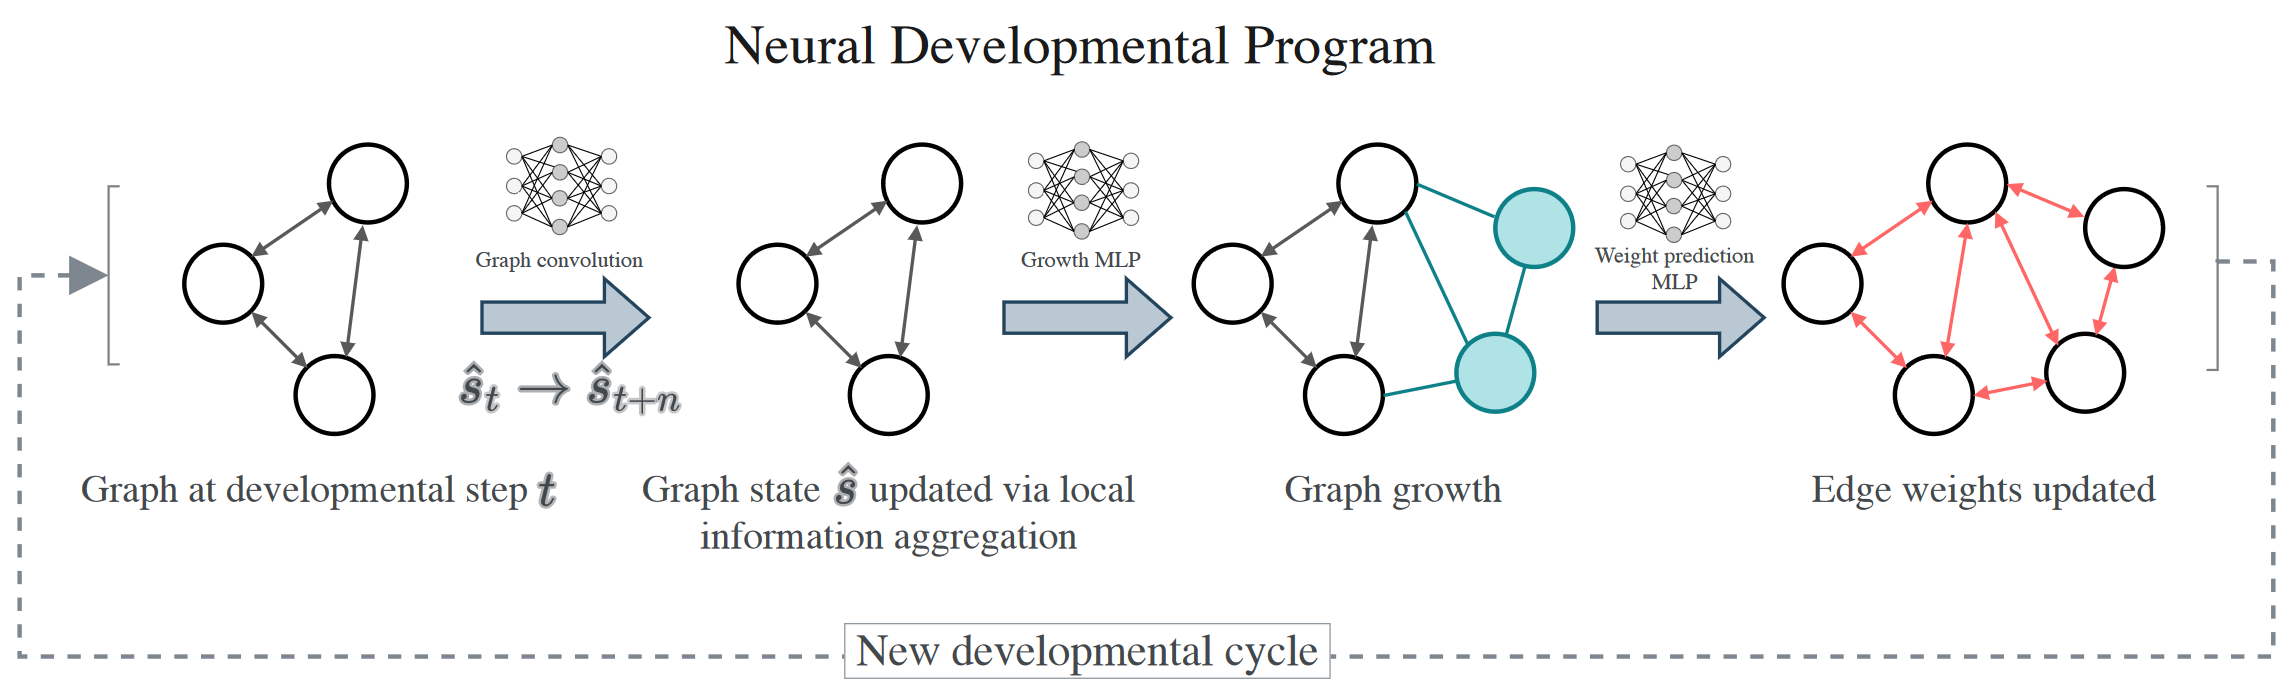
\includegraphics[width=\textwidth]{Fig/2024.7.19_1.png}
    \caption{Neural Development Program approach for growing neural network}
    \label{fig:my_label}
\end{figure}
\begin{itemize}
    \item Use the Neural Development Program(NDP) to control \textbf{the growth of new networks}
    \item Two training methods: \textbf{Evolutionary-based} and \textbf{Gradient-based}
    \item Execute experiments on \textbf{MNIST, XOR, CartPole, LunarLander}
\end{itemize}
\end{frame}

\begin{frame}{July 19, 2024}
    \begin{figure}
        \centering
        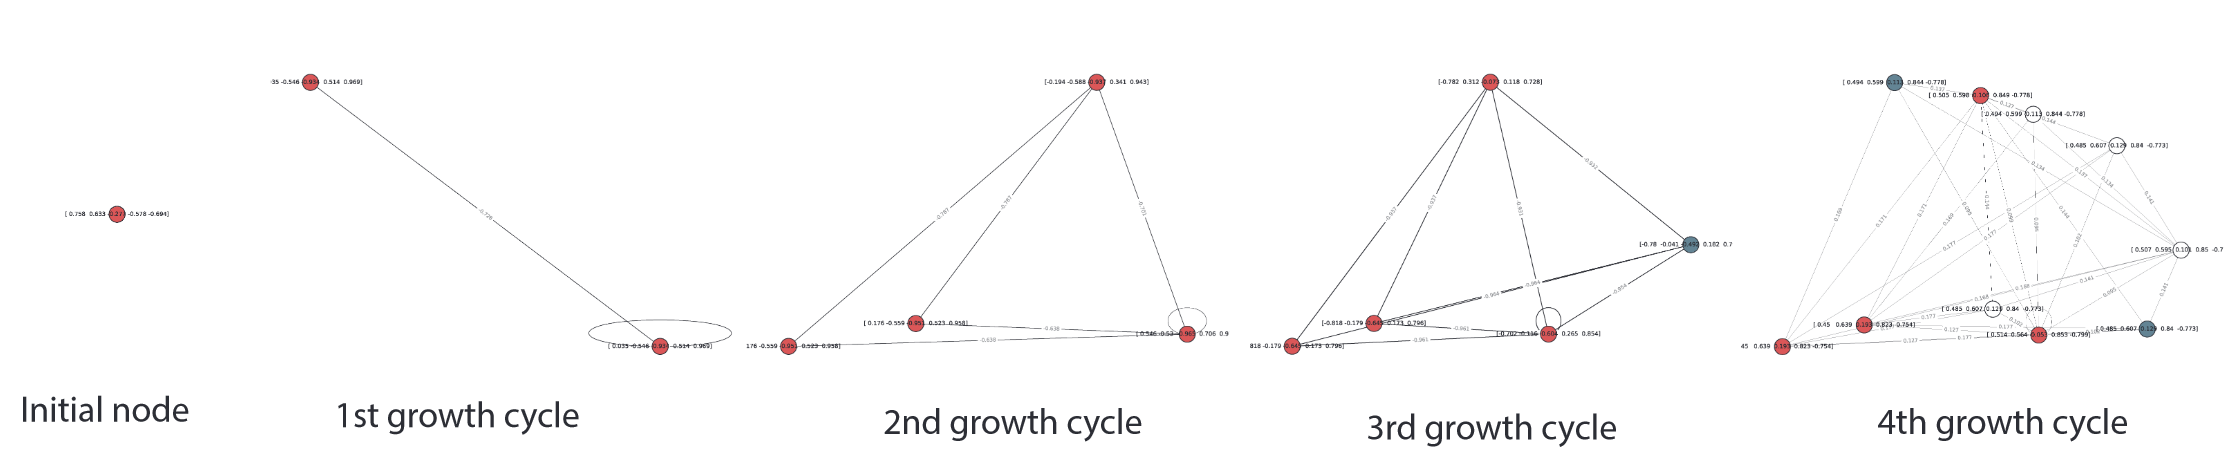
\includegraphics[width=\textwidth]{Fig/2024.7.19_2.png}
        \caption{Developmental growth of the network capable of solving the CartPole balancing task}
        \label{fig:my_label}
    \end{figure}
    \begin{itemize}
        \item No indication of \textbf{robustness} or other performance advantages
        \item No additional information about the \textbf{topological properties} of the network
    \end{itemize}
\end{frame}

\begin{frame}{July 19, 2024}
    \textbf{HYPERNETWORKS}
    \begin{itemize}
        \item An approach of using a \textbf{hypernetwork} to generate the weights for another network, which is similar to the nature: the relationship between a \textbf{genotype} and a \textbf{phenotype}
        \item Generate weights for practical architectures by taking layer embedding vectors as inputs
        \item Hypernetworks are trained \textbf{end-to-end} with gradient descent together with the main network 
    \end{itemize}
    \textbf{Reflection}
    \begin{itemize}
        \item The focus is not on generating networks, but on \textbf{the ability to self-explore} in a multi-task environment
        \item Generative networks are a means of implementation. Are there any existing methods that can achieve self-exploration capabilities to a certain extent, such as \textbf{LLM-based agents}
    \end{itemize}
\end{frame}

\begin{frame}{July 26, 2024}
    \begin{itemize}
        \item Agents environments setup
        \begin{itemize}
            \item New reasoning framework (modify the prompts)
            \item Digital tasks (fine tune on the digital tasks)
            \item Embodied tasks (usually with a vision module)
        \end{itemize}
        \item Learn of reinforcement learning
    \end{itemize}
\end{frame}{}

\begin{frame}{July 26, 2024}
    \textbf{AgentGym}
    \begin{figure}
        \centering
        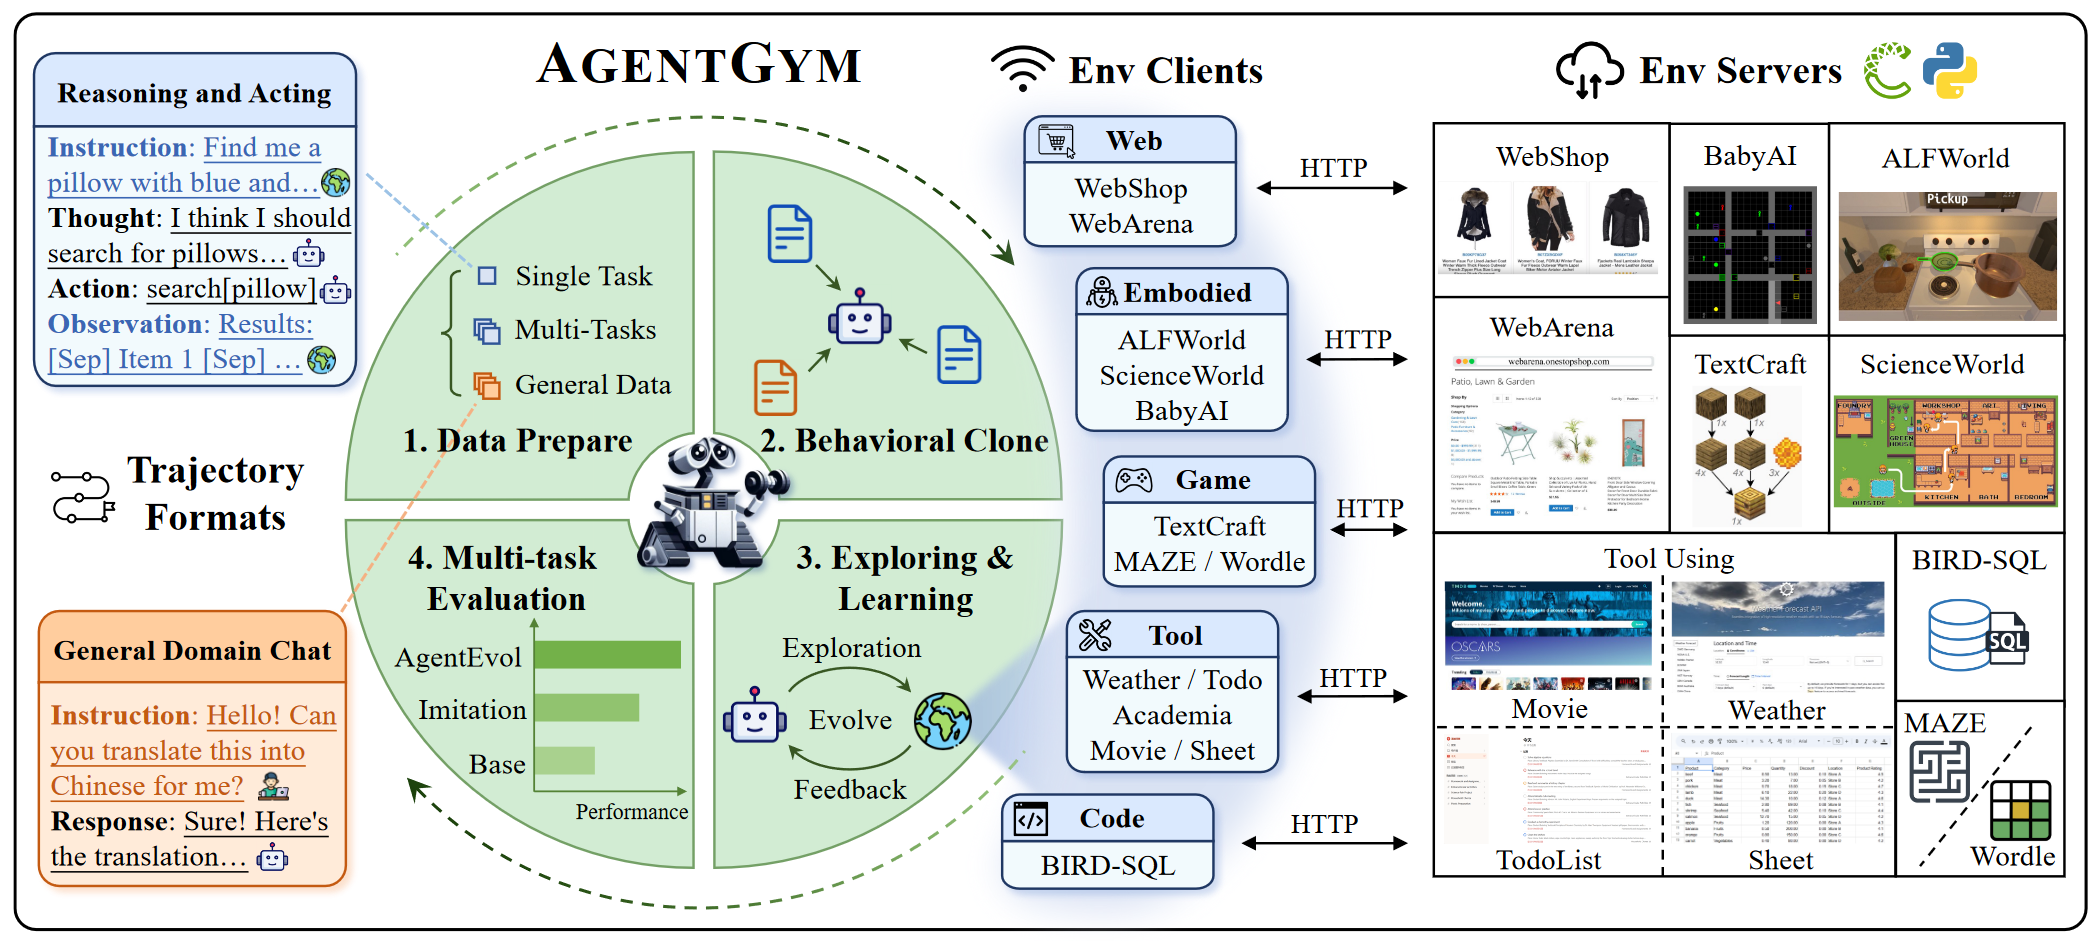
\includegraphics[width=\textwidth]{Fig/2024.7.26_3.png}
        \caption{Overview of the AgentGym framework}
        \label{fig:my_label}
    \end{figure}
\end{frame}

\begin{frame}{July 26, 2024}
    \textbf{OSWORLD}
    \begin{figure}
        \centering
        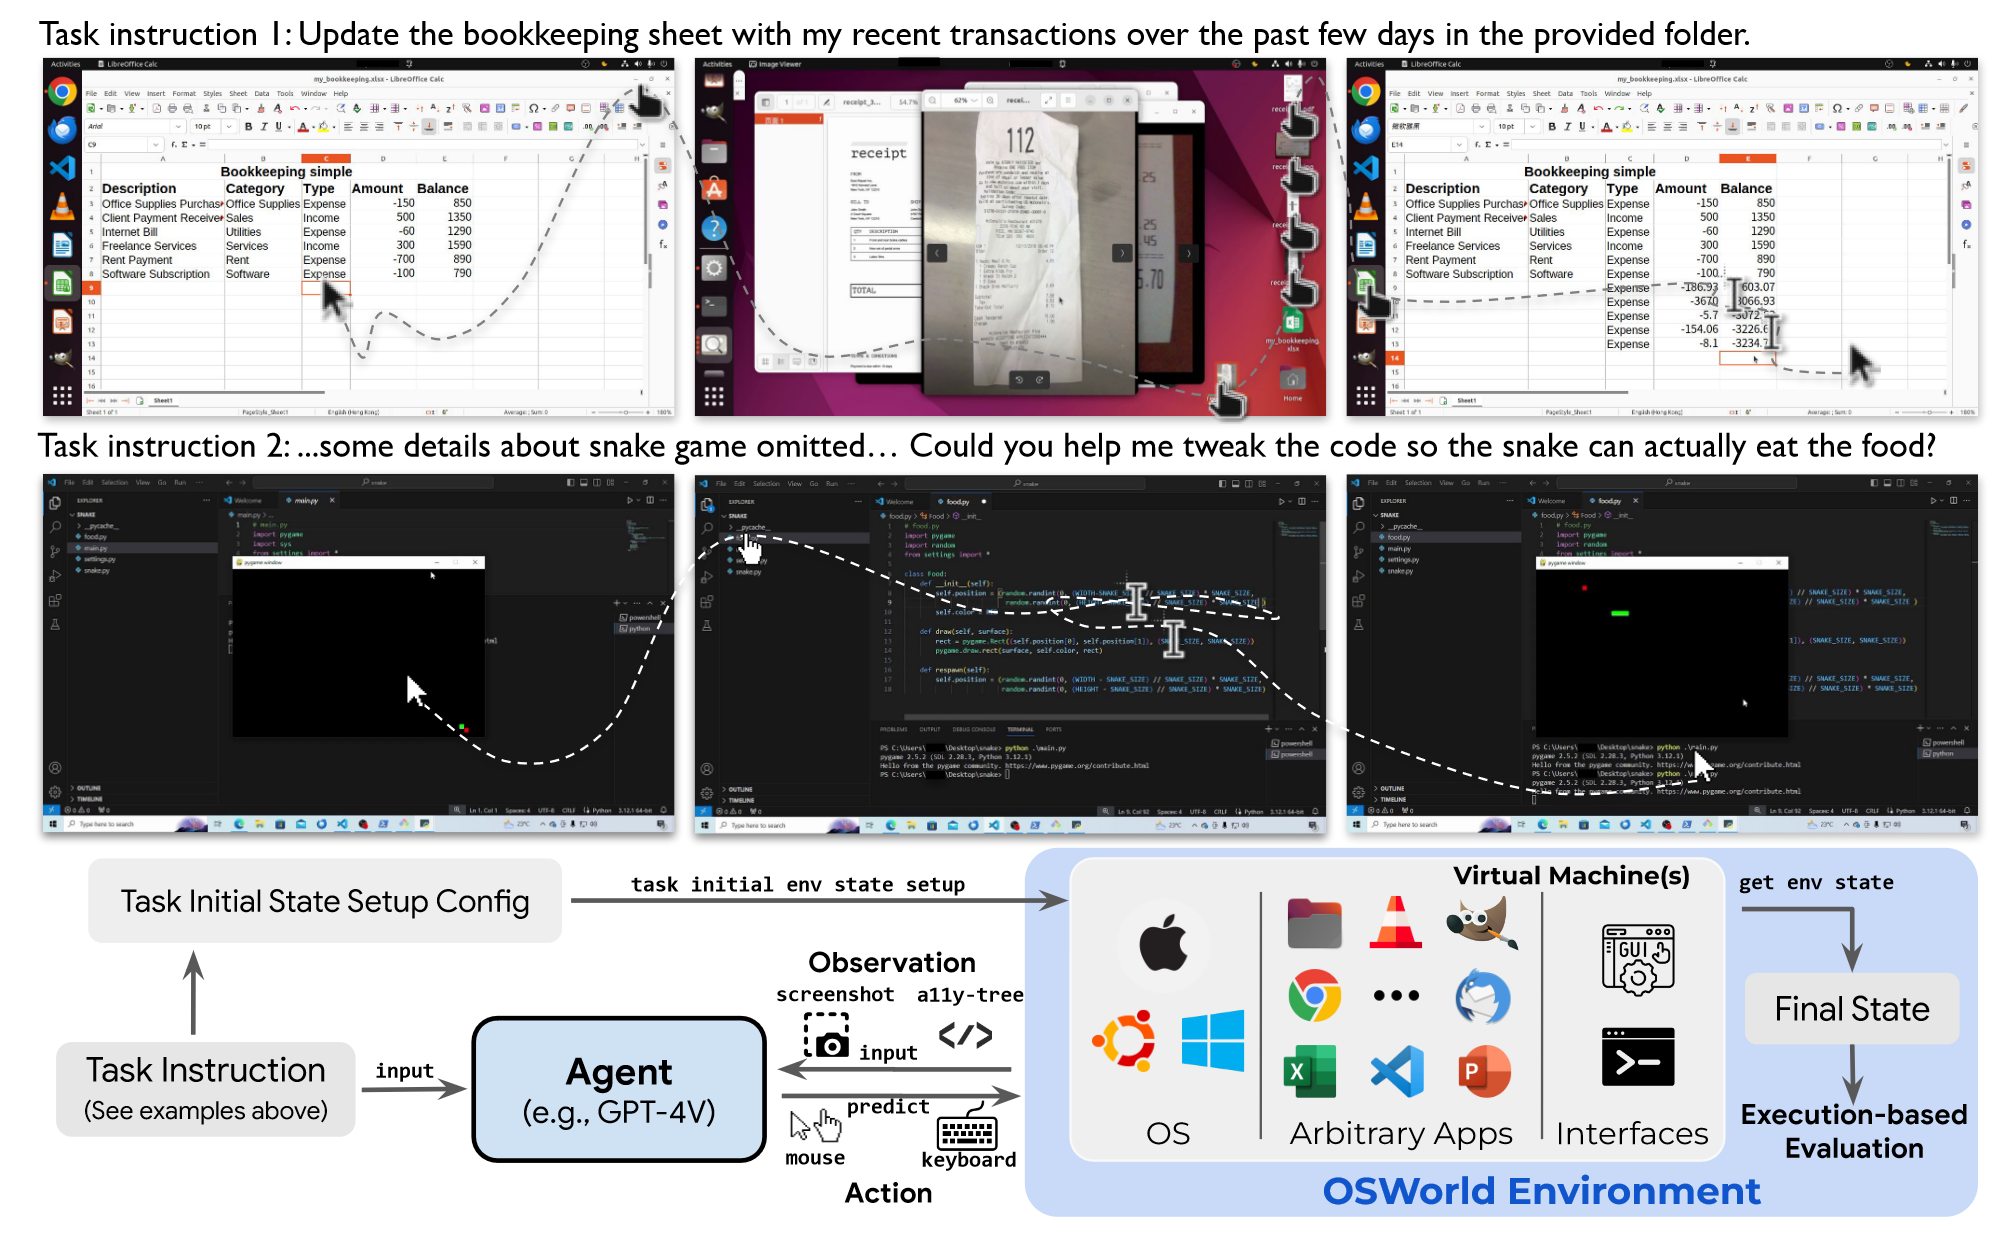
\includegraphics[width=\textwidth]{Fig/2024.7.26_2.png}
        \caption{OSWORLD, a real computer environment for multimodal agents}
        \label{fig:my_label}
    \end{figure}
\end{frame}

\begin{frame}{July 26, 2024}
    \textbf{FunSearch}
    \begin{figure}
        \centering
        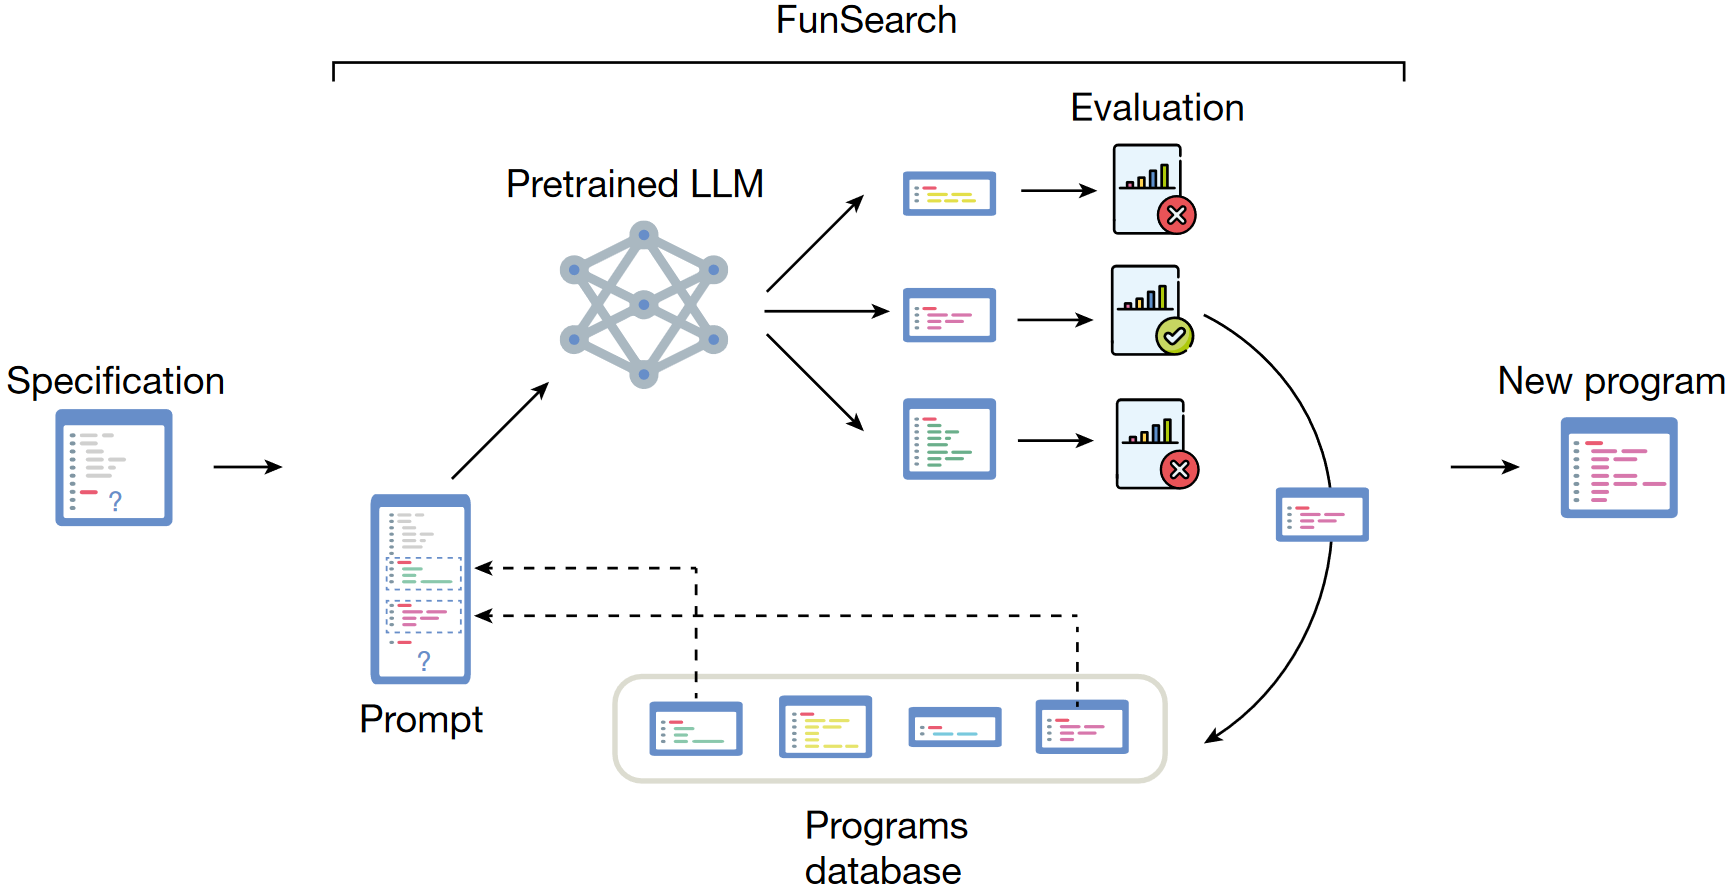
\includegraphics[width=\textwidth]{Fig/2024.7.26_1.png}
        \caption{Overview of FunSearch}
        \label{fig:my_label}
    \end{figure}
\end{frame}

\begin{frame}{Aug. 2, 2024}
\textsc{Target}
    \begin{itemize}
        \item Diffusion Models as Tools for Gene Expression —— Genotype
        \item Use partial modules in a large model to adapt to different tasks —— Phenotype
    \end{itemize}
    \begin{figure}
            \centering
            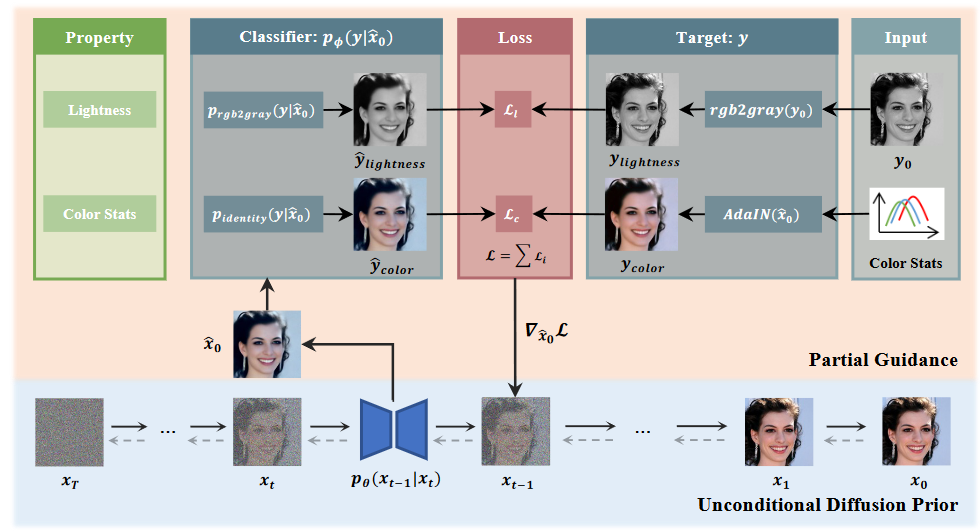
\includegraphics[width=0.7\textwidth]{Fig/2024.8.02_1.png}
            \caption{Overview of Our PGDiff Framework for Versatile Face Restoration}
            \label{fig:my_label}
    \end{figure}
\end{frame}

\begin{frame}{Aug. 2, 2024}
\textsc{Keywords}
\begin{itemize}
    \item Conditional Diffusion Model
    \item Pruning
    \item Model Selector
    \item Multi-task Learning
    \item Neural Architecture Search
    \begin{itemize}
        \item The representations of the architectures in the search space
        \item Introduce diffusion models as a search algorithm
    \end{itemize}
\end{itemize}
\end{frame}

\begin{frame}[standout]
  Questions?
\end{frame}


\end{document}
